\documentclass[10pt,a4paper]{report}
\usepackage[utf8]{inputenc}
\usepackage{amsmath}
\usepackage{amsfonts}
\usepackage{amssymb}
\usepackage{graphicx}
\usepackage{lmodern}
\usepackage{float}
\usepackage[left=2cm,right=2cm,top=2cm,bottom=2cm]{geometry}

\author{Yapi Donatien Achou}
\title{Factors influencing accuracy of the hold up equation}
\begin{document}
\maketitle
\section{Accuracy analysis of the hold up equation}
The dimensionless hold up equation is given by 
\begin{equation}\label{h}
X^{2}F(\tilde{h})-G(\tilde{h},\theta) +4Y = 0
\end{equation}
where $X^{2}$ is the Lockhart-Martinelli parameter and $Y$ is the gravitational parameter. Equation (\ref{h}) is solved for the equilibrium liquid height $\tilde{h}$ at witch the pressure gradient in the liquid is equal to the pressure gradient in the gas. Solutions of (\ref{h}) for $\theta = 1$
is given by the figure bellow

\begin{figure}[H]
  \caption{Equilibrium liquid height from the hold up equation.}
  \centering
    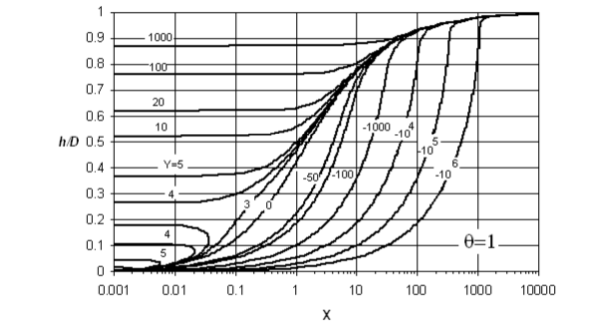
\includegraphics[width=1\textwidth]{hup.png}
\end{figure}
The hold up equation is obtained from the momentum equations, in witch the wall shear stress in each phase is approximated by the hydraulic model:
\begin{equation}
\tau_{wk} = \frac{1}{8}\rho_{k} \bar{U_{k}}^{2}f_{k} \nonumber
\end{equation}
where $f$ is the friction factor. Since the hydraulic model uses the average velocity in the flow direction, all cross sectional information about the velocity field is removed. In addition all information of the velocity gradient governing wall and interfacial stress is lost. Therefore Approximating the wall shear stress by using the hydraulic model will affect the accuracy of the result shown in figure 1.\\
\\
For $\theta = 1$ the interfacial shear stress is given by the shear stress of the gas
\begin{equation}
\tau_{I} = \tau_{Gw}=\frac{1}{8}\rho_{G} \bar{u}_{G}^{2}f_{G}\nonumber
\end{equation}
This does not takes into account the coupling of the gas and the liquid and can affect the accuracy of the result obtained in figure 1.\\
\\
The friction factor for each phase is given by
\begin{equation}
f_{k} = \frac{C_{k}}{R^{n}_{e_{k}}} \nonumber
\end{equation}
hence the single phase friction factor is used in the two phase system. This can affect the accuracy of the result in figure 1.




\end{document}